\usetikzlibrary{trees}
\coversection{Automaten/finit1.png}{Formale Grammatiken}{\\ \hspace*{\fill} - ChatGPT}
\paragraph*{Idee:} Konstruktion aller Wörter einer Sprache.
\paragraph*{Beispiel:} 
\begin{itemize}
    \renewcommand{\labelitemi}{} % Remove bullet point

    \item \(L=\{0^n\}_{n\in\mathbb{N}_0}\)
    \item S Startsymbol
    \item \(S\to \lambda, \ S\to 0S\) Regel \( \quad (S, \lambda), (S, 0S)\)
    \item \(S\to 0S\to 00S\to 000S\to 000\)


\end{itemize}
\mysubsection{Definition (Grammatiken)}
    Eine Grammatik ist ien Tupel \(G=(N,T,P,S)\). Dabei ist 
    \begin{itemize}
        \item N das Alphabet der \textbf{Nichtterminalsymbole/Variablen} 
        \item T das Alphabet der \textbf{Terminalsymbole} mit \(N\cup T=\varnothing \)
        \item \(P\subseteq((N\cup T)^*\backslash T^*)\times (N\cup T)^*\) eine endliche Menge von \textbf{Regeln/Produktionen}, wobei wir für ein Paar \((u, v) \in P\) auch \( u \to v\) schreiben.
        \item \(S\in\mathbb{N}\) das \textbf{Startsymbol}
    \end{itemize}
    Eine \textbf{Satzform} von G ist ein Wort \(s\in(N\cup T)^*\) und eine \textbf{Terminalwort} von G ist ein Wort \(t\in T^*\).
\mysubsection{Definition (Ableitung)}
    Sei \(G=(N,T,P,S)\) eine Grammatik. Eine Satzform \(w'\) von G ist in einem Schritt aus einer Satzform w von G \textbf{ableitbar}, wenn es Satzformen u,v,x,y von G gibt, so dass \(w=xuy,u\to v\in P\) und \(w'=xvy\) gelten. Es bezeichne \(\to_G\) die Relation auf der Menge der Satzformen von G, sodass \(w\to_Gw'\) genau dann für Satzformen von G gilt, wenn w' aus w in einem Schritt ableitbar ist.\\
    Für Satzformen u,v von G ist eine \textbf{Ableitung} von v aus u eine Folge \(u=w_1,\cdots,w_n=v\) mit \(w_i\to_Gw_{i+1}\) \(\forall i\in[n-1]\) und eine Ableitung von v in G ist eine \textbf{Ableitung} von v aus S in G. Für \(n\in\mathbb{N}\) schreiben wir \(u\to^n_Gv\) wenn es eine Ableitung von $v$ aus $u$ der Länge $n$ gibt und wir schreiben \(u\to^*_Gv\) wenn eine Ableitung von v aus u in G existiert.\\\\
    \textit{Erklärung:}\\
    Stell dir vor, du möchtest ein Rezept zum Backen von Kuchen haben. Das Rezept besteht aus verschiedenen Schritten, wie zum Beispiel das Mischen der Zutaten und das Backen im Ofen. In ähnlicher Weise kann man sich eine Grammatik vorstellen, die Regeln für den Aufbau von Sätzen in einer Sprache festlegt.
    Nehmen wir an, du hast eine Grammatik namens G, die aus Buchstaben (N) und Wörtern (T) besteht. Diese Grammatik hat auch Regeln (P) und einen Startpunkt (S). Eine Satzform ist ein Satz, der in der Grammatik G gebildet werden kann.
    Jetzt stellen wir uns vor, du hast einen Satz, den wir als "w" bezeichnen. Du möchtest einen anderen Satz, "w'", in einem Schritt aus dem Satz "w" ableiten. Das bedeutet, dass es bestimmte Regeln gibt, die angewendet werden können, um von "w" zu "w'" zu gelangen. Man kann sich das wie einen Schritt in einem Rezept vorstellen, bei dem man eine Zutat durch eine andere ersetzt oder sie anders kombiniert.
    Eine Ableitung ist eine Folge von Schritten, bei der man von einem Satz "u" zu einem anderen Satz "v" gelangt. Jeder Schritt in der Ableitung wird durch eine Regel aus der Grammatik G dargestellt. Eine Ableitung von "v" in G ist eine Ableitung von "v" ausgehend vom Startpunkt "S" in G.
    %Um die Länge einer Ableitung anzugeben, verwenden wir die Zahl "n". Wenn wir schreiben "u ->^n_G v", bedeutet das, dass es eine Ableitung von "v" aus "u" gibt, die aus genau "n" Schritten besteht. Wenn wir schreiben "u ->^*_G v", bedeutet das, dass es eine Ableitung von "v" aus "u" in G gibt.
    
    
\mysubsection{Definition (Erzeugte Sprache)}
    Sei \(G=(N,T,P,S)\) eine Grammatik. Die von G erzeugte Sprache \(L(G)\) ist die Menge aller Wörter \(w\in T^*\) für die es eine Ableitung von w in G gibt.
\mysubsection{Lemma} 
    Sei \(G=(N,T,P,S)\) eine Grammatik und seien u,v,x,y Satzformen von G und seien \(n,m\in\mathbb{N}\) mit \(u\to_G^nv\) und \(w\to_u^nxuy\).\\
    Dann gilt \(w\to_u^{m+n-1}xvy\).
\begin{proof}
    Sei \(\alpha _1,\cdots,\alpha_n\) ein Ableitung von xuy aus w und \(\beta_1,\cdots,\beta_m\) eine Ableitung von v aus u. Dann ist\\ 
    \(\alpha_1,\cdots,\alpha_{n-1},x\beta_1y,\cdots,x\beta_my=xvy\)\\
    eine Ableitung von xvy aus w in G der Länge n+m-1.\par\bigskip
    Im folgenden beschäftigen wir uns mit dem Thema welche Sprache Grammatiken verschiedener Komplexitätsstufen erzeugen können.
\end{proof}

\mysubsection{Satz}
    Eine Sprache ist genau dann rekuriv aufzählbar, wenn sie von einer Grammatik erzeugt wird.
\paragraph*{Beweisidee} 
    Wird eine Sprache $L$ von einer Grammatik erzeugt, so ist $L$ die erkannte Sprache einer TM, die in geeigneter Weise Ableitungen von $G$ erzeugt, prüft ob diese Ableitung dem Wort der Eingabe entspricht und gegebenfalss akzeptiert. Wenn eine Ableitung der Eingabe gefunden ist.\par\bigskip
    Gegeben eine rekursiv aufzählbare Sprace $L$ und eine TM, die $L$ erkennt. So konstruieren wir ähnlich dem Postschen Korrespondenzproblems Regeln und Symobole, sodass wir die Arbeitsweise der TM modellieren können und entsprechend mit einem Terminalwort enden wenn dies von der TM erkannt wird.
\mysubsection{Definition (Rechtslinear)}
    Eine Grammatik \(G=(N,T,P,S)\) ist rechtslinear, wenn alle Regeln von der Form 
    \[X\in uy \text{ oder } X\to u\]
    mit \(X,y\in\mathbb{N}\) und \(u\in T^*\) sind.\par\bigskip 
    Hier ist es sinnvoll endliche Automaten zu betrachten bei denen es nicht \(\forall\) Zustände q und Eingabesymbole a ein Tripel \((q,a,q')\) in der Übergangsrelation geben muss. Solche Automaten sind zwangsläufig nicht deterministisch.
\mysubsection{Satz}
    Eine Sprache ist genu dann regulär, wenn sie von einer rechtslinearen Grammatik erzeugt wird.
\paragraph*{Beweisidee}
    Zunächst überzeugt man sich davon, dass eine Sprache L genau dann von einer rechtlinearen Grammatik erzeugt wird, wenn sie von einer Grammatik \(G=(N,T,P,S)\) erzeugt wird bei der alle Regeln von der Form \(X\to ay\) oder \(X\to \lambda\)\\
    mit \(x,y\in\mathbb{N}\) und \(a\in T\) sind. Eine Solche Grammatik wird als Grammatik in Simulationsform bezeichnet.\par\bigskip
    Die Sprache L die von einer rechtslinearen Grammatik (in Simulationsform) gebildet wird von dem EA 
    \[
        A=(N,T,\Delta,S,\{X\in N: X\to \lambda\in P\})
    \]
    mit 
    \[
        \Delta=\{(X,a,y)\in N\times T\times N:X\to ay\in P\}
    \]
    erkannt.\\
    Umgekehrt ist es einfach zu sehen, dass jede Reguläre Sprace von einer rechtslinearen Grammatik erzeugt wird. 

\mysubsection{Beispiel}
    Die Sprache \(\{0\}^*\) wird von der rechtlinearen Grammatik \[ G = (\{S\},\ \{0,\ 1\}^*,\ \{S \to 0S,\ S \to \lambda\},\ S)\] erzeugt von EA \[A = (\{S\},\ \{0,\ 1\}^*,\ \{(S,\ 0,\ S)\},\ S, \{S\})\] erkannt. Sowohl auf der Seite der Machinenmodelle als auch auf der Seite der Grammatiken gibt es weitere wichtige Sprachklassen, die sich ergeben wenn der Maschinenarbeitsweise oder Menge der zulässigen Regeln weniger stark eingeschränkt wird bei EA und rechtslinear Grammatiken.

\mysubsection{Definition (kontextfrei)} 
    Eine Grammatik \(G = (N,\ T,\ P,\ S)\) ist \textbf{kontextfrei}, wenn alle Regeln von G von der From \[X \to w\] mit \(X \in N\) und \(w \in (N \cup T)^*\) sind. Eine Sprache ist \textbf{kontextfrei}, wenn sie von einer Kontextfreien Grammatik erzeugt wird. Die Menge aller kontextfreien Sprachen bezeichnen wir mit \textbf{CF}.

\mysubsection{Definition (lexikographische Ordnung)}
    Sei \(\Sigma \) ein Alphabet. Die \textbf{lexikographische Ordnung} aud \(\Sigma^*\) ist die lineare Ordnung \(leq\) aud \(\Sigma^*\) für doe \(u \leq v\) für \(u, v \in \Sigma^*\) genau dann gilt wenn eine der folgenden Bedingungen erfüllt ist.
    \begin{itemize}
        \item [(L1)] \( u \sqsubseteq v\).
        \item [(L2)] Es gibt ein \(i \in [min \{|u|, |v|\}] \) mit \( u(j) = v (j) \quad \forall j \in [i - 1]\) und \(u (i) \not = v (i)\) und \(u (i) \leq v(i)\) für eine gebildete, lineare Ordung \(\leq\) auf \(\Sigma\)
    \end{itemize}
    Schreiben wir \(\leq\) für eine lineare Ordnung, so bedeutet \(u < v\) für Elemente \(u, v\), dass \(u \leq v\) und \(u \not = v\) gelten.
    \newpage
    Betrachte \(G = (\{S, X\}, \{0, 1\}, P, S)\) mit \[P = \{S \to XX,\ X \to 0X1,\ X \to \lambda\}\] 
    Betrachte Ableitung \(S,\ XX, X0X1,\ 0x10x1,\ 0X101,\ 00X1101,\ 001101\)
    \vspace{1cm}
    \createDiagram{}
    {
        \begin{tikzpicture}[level distance=2cm,
            level 1/.style={sibling distance=5cm},
            level 2/.style={sibling distance=2cm}]
            
            \node {S}
            child 
            {
                node {X}
                child{node {0}}
                child 
                {
                    node {X}
                    child {node {0}}
                    child 
                    {
                        node{X}
                        child{node {$\lambda$}}
                    }
                    child{node {1}}
                }
                child {node {1}}
              }
              child 
              {
                node {X}
                child 
                {
                    node {0}
                }
                child 
                {
                    node {X}
                    child 
                    {
                        node {$\lambda$}
                    }
                }
                child 
                {
                    node {1}
                }
            };
              
            \node[right=1cm] at (current bounding box.east) 
            {
                \begin{minipage}{6cm}
                    \begin{itemize}
                        \item oben Wurzel
                        \item die Ordnung der Knoten/ Ecken ist wichtig
                        \item Knoten/ Ecken haben Beschriftungen
                    \end{itemize}
                \end{minipage}
            };
        \end{tikzpicture}
    }
    \begin{center}
        
    \end{center}
    \createDiagram{}
    {
        \begin{tikzpicture}[level distance=2cm,
        level 1/.style={sibling distance=5cm},
        level 2/.style={sibling distance=2cm}]
        
            \node {$\lambda$}
            child 
            {
                node {1}
                child{node {11}
                    child{node {111}}
                    child{node {112}}
                }
                child{node {12}}
            }
            child 
            {
                node {2}
                child{node {21}}
            }
            child 
            {
                node {3}
                child{node {31}}
                child{node {32}}
                child{node {33}}
            };
        \end{tikzpicture}
    }
    \begin{itemize}
        \item Abbildung 12 repräsentiert die Sprache $T = \{\lambda, 1, 2, 3, 11, 12, 21, 31, 32, 33, 111, 112\}$.
        \item Der Wurzelknoten ist $\lambda$.
        \item Die Reihenfolge ist lexikographisch.
    \end{itemize}
    
\mysubsection{Definition (Baum)} 
    Eine endliche nicht leere Sprache T heißt \textbf{Baum}, wenn sie unter Präfixbildung abgeschlossen ist, also wenn für alle \(w \in T\) und \(p \sqsubseteq w\) auch \(p \in T\) gilt. Ein Wort \(w \in T\) heißt \textbf{Blatt} von T, wenn w bezüglich \(\sqsubseteq \) maximal in T istm also wenn \(w = w' \quad \forall w' \in T\) mit \(w \sqsubseteq w'\) gilt. Wörter \(w \in T\), die keine Blätter von T sind heißen \textbf{innere Ecken} von T.

\mysubsection{Lemma}
    Sei \(\Sigma\) eine Alphabet und \(\leq\) die lexikographische Ordnung auf \(\Sigma^*\). Seien \(u, w \in \Sigma^*\) mit \(u \not \sqsubseteq w\) und \(u \leq w\). Seien \(v_1<\cdots<v_n \in \Sigma^*\) mit \(v_1 \not = \lambda\). Dann gilt \(u < u v_1< \cdots < uv_n < w\)

    \createDiagram{Baum und Präfixbildung}
    {
        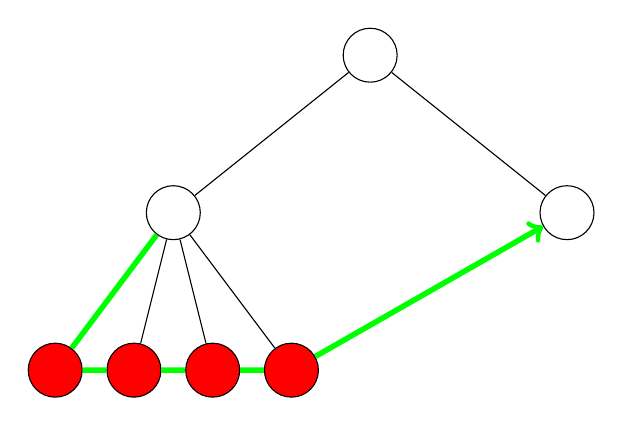
\begin{tikzpicture}[level distance=2cm,
            level 1/.style={sibling distance=5cm},
            level 2/.style={sibling distance=1cm},
            circleNode/.style={circle, draw, minimum size=1.5em}]

            \node [circle,draw]{\phantom{X}}
            child 
            {
                node [circle,draw](node1){\phantom{X}}
                child{node [circle,draw, fill=red](node2){\phantom{X}}}
                child{node [circle,draw, fill=red](node3){\phantom{X}}}
                child{node [circle,draw, fill=red](node4){\phantom{X}}}
                child{node [circle,draw, fill=red](node5){\phantom{X}}}
            }
            child 
            {
                node [circle,draw](node6){\phantom{X}}
            };

            \draw[->, draw=green, line width=2pt] (node1) -- (node2) -- (node3) -- (node4) -- (node5) -- (node6);
        \end{tikzpicture}
    }

    \begin{proof}
        Für \(v, v' \in \Sigma^*\) mit \(v \leq v'\) gilt offenba \(uv \leq uv'\)m es genügt also zu zeigen, dass \(uv \leq w \quad \forall v \in \Sigma^*\) gilt. Wegen \(u \not \sqsubseteq w\) existiert \(i \in [min \{|u|, |w|\}]\) mit \(u(j) = w(j) \quad \forall j \in [i-1]\) und \(u(i) < w(i)\). Für \(v \in \Sigma^*\) gilt dann \((uv)(j)=w(j) \quad \forall j \in [i - 1]\) und \((uv)(j)<w(i)\), also \(uv < w\).
    \end{proof}

\newpage

\mysubsection{Lemma}
    Sei T ein Baum, \(\leq\) die lexikographische Ordnung auf T, \(p \in T\) und \(Q:=\{w\in T: p\sqsubseteq w\}\). Es gelten \(p = min Q\) und \(Q = \{w \in T : min Q \leq w \leq max \leq max Q\}\). 

    \createDiagram{}
    {
        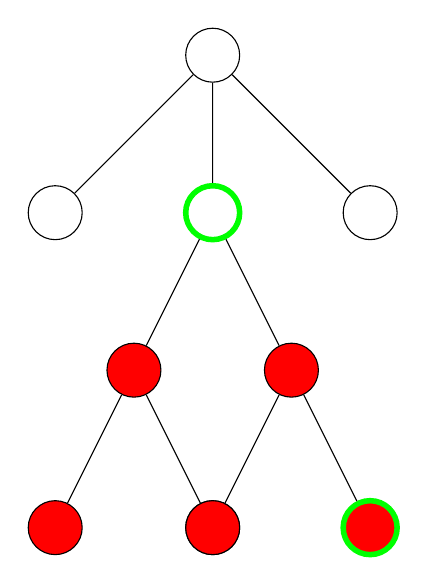
\begin{tikzpicture}[level distance=2cm,
            level 1/.style={sibling distance=2cm},
            level 2/.style={sibling distance=2cm}]
            
            \node [circle,draw]{\phantom{X}}
            child 
            {
                node [circle,draw]{\phantom{X}}
              }
              child 
              {
                node [circle,draw = green, line width=2pt]{\phantom{X}}
                child 
                {
                    node [circle,draw, fill = red]{\phantom{X}}
                    child 
                    {
                        node [circle,draw, fill = red]{\phantom{X}}
                    }
                    child 
                    {
                        node [circle,draw, fill = red]{\phantom{X}}
                    }
                }
                child 
                {
                    node [circle,draw, fill = red]{\phantom{X}}
                    child 
                    {
                        node [circle,draw, fill = red]{\phantom{X}}
                    }
                    child 
                    {
                        node [circle,draw = green, fill = red, line width=2pt]{\phantom{X}}
                    }
                }
            }
            child
            {
                node[circle,draw][circle,draw]{\phantom{X}}
            };
        \end{tikzpicture}
    }
    \begin{proof}
        Offensichtlich gilt \(p = min Q\). Für \(w \in Q\) gilt \(min Q \leq w \leq max Q\) nach Definition von min Q und max Q. Für \(w \not \in Q\) mit \(w \sqsubseteq w' \quad \forall w' \in Q\), also \(w < min Q\). Für \(w \not \in Q\) mit \(w \not \sqsubseteq p \quad \exists i \in [min {|p|, |w|}]\) mit \(w(i) \not = p(i)\), insbesondere existiert also ein minimales solches i und nach Definition von \(\leq\) folgt damit \(w \leq w' \quad \forall w'\in Q\) oder \(w' \leq w \quad w' \in Q\), insbesondere also wegen \( w \not \in Q\) somit \( w < min \ Q\) oder \(max \ Q < w\).
    \end{proof}

\mysubsection{Definition (Beschriftung)} 
    Eine \textbf{Beschrftung} eines Baumes T mit Elementen einer Menge X ist eine Funktion \(b: T \to X\).

\newpage

\mysubsection{Definition (Blattwort)}
    Sei \(\Sigma\) eine ALphabet, sei (T,b) ein Paar aus einem Baum T und einer Beschrifung \(b: T \to \Sigma \cup \{\lambda\}\) und sei \(t_1, \cdots, t_n\) dieFolge der Blätter von T in lexikographischer Reihenfolge. Das \textbf{Blattwort} von (T, b) ist \(b(t_1) \cdot b(t_n)\). Blattwort: 001101
    \createDiagram{Blattwort}
    {
        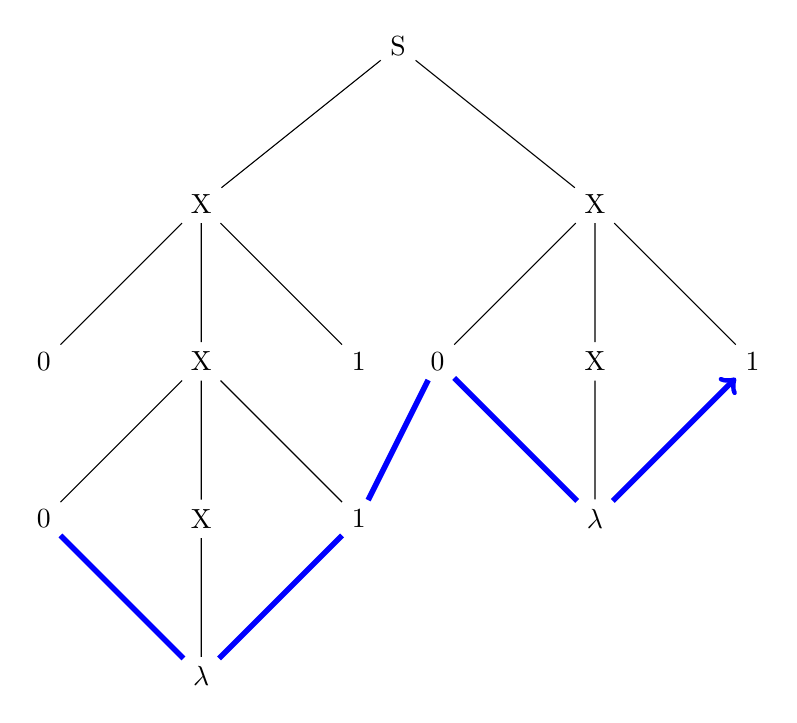
\begin{tikzpicture}[level distance=2cm,
            level 1/.style={sibling distance=5cm},
            level 2/.style={sibling distance=2cm}]
            
            \node (node1) {S}
            child 
            {
                node (node2) {X}
                child{node (node3) {0}}
                child 
                {
                    node (node4){X}
                    child {node (node5){0}}
                    child 
                    {
                        node (node6){X}
                        child{node (node7) {$\lambda$}}
                    }
                    child{node (node8) {1}}
                }
                child {node (node9) {1}}
              }
              child 
              {
                node (node10) {X}
                child 
                {
                    node (node11) {0}
                }
                child 
                {
                    node (node12){X}
                    child 
                    {
                        node (node13){$\lambda$}
                    }
                }
                child 
                {
                    node (node14){1}
                }
            };
            \draw[->, draw=blue, line width=2pt] (node5) -- (node7) -- (node8) -- (node11) -- (node13) -- (node14);

        \end{tikzpicture}
    }
\newpage
\mysubsection{Definition (Ableitungsbaum)} 
    In einer kontextfreien Grammatik \(G = (N,\ T,\ P,\ S)\) ist ein \textbf{Ableitungsbaum} für eine Satzform \(w \in (N \cup T)^*\) aus \(A \in N\) ein paar (T, b), bestehend aus einem Baum T und einer Beschriftung \(b: T \to N \cup T \cup \{\lambda\}\). Der baum T ist eine Teilmenge von \([d]^*\), wobei \(d:= max (\{|w|: x \to w \in P\} \cup \{1\})\). Die Wurzel des baumes ist mit dem Symbol A beschriftet und das Blattwort entspricht der Satzform w. Für jede innere Ecke t im Baum T existiert eine Regel \(X \to v \in P\), sodass Folgendes gilt.    \footnote{Tex. Ed. sug.}
    \begin{itemize}
        \item [(i)] \(b(t) = X\)
        \item [(ii)] \(\{t' \in T : t \sqsubseteq t' \text{ und } |t'| = |t| + 1\} = \{ta : a \in max \{|v|, 1\}\}\)
        \item [(iii)] \(b(ta) = v(a) \quad \forall a \in [|v|]\)
        \item [(iv)] \(b(t_1) = \lambda \text{ falls } v = \lambda\)
    \end{itemize}
    Die \textbf{Blätter} von (T, b) sind die Blätter von T und die \textbf{inneren Ecken} von (T, b) sind die inneren Ecken von T.

\mysubsection{Beispiel}     
    Sei \(G = (\{S\},\ \{0,\ 1\},\ \{S \to 0S1,\ S \to \lambda\},\ S),\ T = \{\lambda,\ 1,\ 2,\ 3,\ 21,\ 22,\ 23,\ 221\}\) und sei \(b:T\to\{S,\ 0,\ 1,\ \lambda\}\) die Beschriftung mit \(b(\lambda) = b(2) = b(22) = S,\ b(1) = b(21) = 0\) und \(b(221) = \lambda\). Dann ist (T, b) ein Ableitungsbaum von 0011 aus S un G. Die \textbf{Darstellung} von T sieht wi folgt aus: \[HIERABBEINFÜGEN\]
    \createDiagram{Darstellung von T}{}

    \[Visualisierung 1 + 2 \]
    \createDiagram{Colorization}{}

    \mysubsection{Lemma}
    Sei \(G = (N,\ T,\ P,\ S)\) eine kontextfreie Grammatik und \(w_1, \cdots, w_l\) eine Ableitung von w aus S in G. Dann gibt es einen Ableitungsbaum (T, b) von w aus S in G mit \(l-1\) innere Ecken. 
    \begin{proof}
        Induktion über l.\\
        \textbf{L = 1} S = (T, b)\\
        Sei nun \(l \geq 2\) und die Aussage wahr \(\forall l' < l\). Sei (T', b') ein Ableitungsbaum von \(w_{l-1}\) aus S in G mit \(l-2\) innere Ecken (existiert per Induktions Hypotese). Sei \(w' := w_{l-1}\). Sei \(i \in [|w'|]\) und \(v \in (N \cup T)^*\) mit \(w'(i) \to v \in P\) und \(w = w'(1) \cdot w'(i-1) v w'(i+1)\cdots w'(|w'|)\). Sei t' das in lexikographischer Reihenfolge i-te Blatt von T' und sei (T, b) der Ableitungsbaum mit \(T = T' \cup \{t'a : a \in [|v|]\},\ b(\tilde{w}) = b'(\tilde{w}) \quad \forall \tilde{w} \in T'\) und \(b(t'a) = v(a) \quad \forall a \in [|v|]\). Aus Lemma 6.12 folgt dann, dass w das Blattwort von (T, b) ist. Außerdem ist die Anzahl der inneren Ecken von T durch \(l - 2 + 1 = l - 1\) gegeben.
    \end{proof}

\mysubsection{Lemma} 
    Sei \(G = (N,\ T,\ P,\ S)\) eine kontextfreie Grammatik und (T, b) ein Ableitungsbaum von w aus S in G mit \(l - 1\) inneren Ecken. Dann gibt es eine Ableitung \(leq = w_1, \cdots\) 
    \[ohne beweis\]


\newpage
\mysubsection{Satz (Pumping-Lemma für kontextfreie Sprachen)}
    Sei \(\Sigma\) ein Alphabet. Für jede kontextfreie Sprache \(L \subseteq \Sigma^*\) gibt es eine Konstante \(\in \mathbb{N}\), so dass folgendes gilt:\\ Ist \(z \in L\) mit \(|z| \geq k\), so gibt es Wörter \(u, v, w, x, y \in \Sigma^*\) mit \(z = uvwxy\), so dass folgendes gilt.
    \begin{itemize}
        \item [(i)] \(vx \not = \lambda\)
        \item [(ii)]\(|vwx| \leq k\)
        \item [(iii)] \(uv'wx'y\in L \quad \forall i \in \mathbb{N}_0\)
    \end{itemize}
    \begin{proof}
            Sei \(G = (N,\ T,\ P,\ S)\) eine kontextfreie Grammatik mit \(L(G) = L\), sei \(d:=max\ (\{|v|: X \to v \in P\} \cup \{1\})\), sei \(k := |[d]|^{\geq |N| + 2}\). Sei \(z \in L\) mit \(|z|\leq k\). Sei (T, b) eine Ableitungsbaum von z aus S in G mit minimaler Anzahl innerer Ecken. Sei \(r \in T \) ein Wort maximaler Länge. Da z Blattwort von T ist folgt insbesondere \(|T| \leq |z| \leq k > |1[d]^{|N|+1}|\), also \(T \not \subseteq [d]^{\geq |\mathbb{N}|+1}\) und somit gilt \(|r|\geq |N|+2\). Seien \(s, t\in[d^*]\) mit \(r = st\) und \(|t| = |N|+2\). Nach schubfachprinzip existieren Präfixe \(t_1, t_2\) von t mit \(b(st_1) = b(st_2)\in N\) und \(|t_1|<|t_2|\). Dann ist auch \(t_1\) Präfix 
    \end{proof}
    \createDiagram{Ableitungsbäume}
    {
        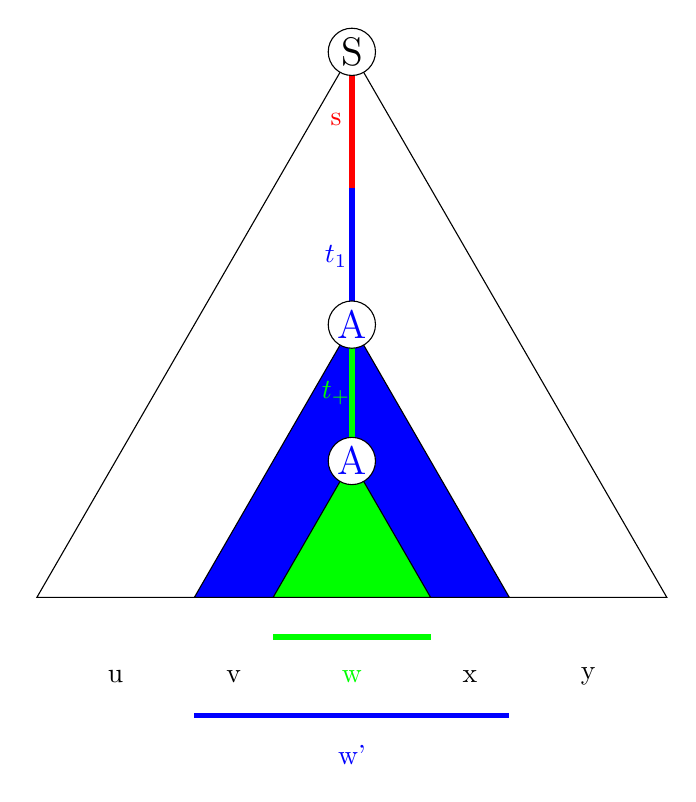
\begin{tikzpicture}

            \coordinate (G) at (-3,0);
            \coordinate (H) at (5,0);
            \coordinate (I) at (1,{4*sqrt(3)});
            \draw[fill=white] (G) -- (H) -- (I) -- cycle;
            \node at (G) [below] {};

            \coordinate (D) at (-1,0);
            \coordinate (E) at (3,0);
            \coordinate (F) at (1,{2*sqrt(3)});
            \draw[fill=blue] (D) -- (E) -- (F) -- cycle;
            \node at (D) [below] {};

            \coordinate (A) at (0,0);
            \coordinate (B) at (2,0);
            \coordinate (C) at (1,{sqrt(3)});
            \draw[fill=green] (A) -- (B) -- (C) -- cycle;
            \node at (A) [below] {};

            \coordinate (M) at (1,{3*sqrt(3)});
            \draw[red, line width=2pt] (I) -- (M);

            \draw[blue, line width=2pt] (M) -- (F);
            \draw[green, line width=2pt] (F) -- (C);


            \coordinate (J) at (1,{4*sqrt(3)});
            \draw[fill=white] (J) circle [radius=0.3];    
            \node at (J) {\Large S};

            \coordinate (K) at (1,{2*sqrt(3)});
            \draw[fill=white] (K) circle [radius=0.3];
            \node at (K) [text=blue]{\Large A};

            \coordinate (L) at (1,{sqrt(3)});
            \draw[fill=white] (L) circle [radius=0.3];
            \node at (L) [text=blue]{\Large A};


            \coordinate (N) at (0.8,{3.5*sqrt(3)});
            \node at (N) [text=red]{s};

            \coordinate (O) at (0.8,{2.5*sqrt(3)});
            \node at (O) [text=blue]{$t_1$};

            \coordinate (P) at (0.8,{1.5*sqrt(3)});
            \node at (P) [text=green]{$t_+$};


            \coordinate (Q) at (-2,-1);
            \node at (Q) {u};
            \coordinate (R) at (-0.5,-1);
            \node at (R) {v};
            \coordinate (S) at (1,-1);
            \node at (S) [text=green]{w};
            \coordinate (T) at (2.5,-1);
            \node at (T) {x};
            \coordinate (U) at (4,-1);
            \node at (U) {y};

            \coordinate (V) at (-1, -1.5);
            \coordinate (W) at (3, -1.5);
            \draw[blue, line width=2pt] (V) -- (W);

            \coordinate (Y) at (0, -0.5);
            \coordinate (Z) at (2, -0.5);
            \draw[green, line width=2pt] (Y) -- (Z);


            \coordinate (X) at (1, -2);
            \node at (X) [text=blue] {w'};

            

        \end{tikzpicture} 
    }
    
    Wir betrachten vier Ableitungsbäume.
    \begin{itemize}
        \item [(1)] Sei \((T_1, b_1)\) des Ableitungsbaum mit \(T_1 = \{q \in [d]^*:s,t,q \in T\}\). Sei w' das Blattwort von \((t_1, b_1)\).\((T_1, b_1)\) ist ein Ableitungsbaum von w' aus A in G.
        \item [(2)] Sei \(T_2, b_2\) der Ableitungsbaum mit \(T_2 = \{q \in [d]^* : st_2q\in T\}\) und \(b_2(q) = b(st_2q \quad \forall q\in T_2)\). Sei \textbf{w} das Blattwort von \(T_2, b_2\). Der Ableitungsbaum \(T_2, b_2\) ist ein Ableitungsbaum von w aus A in G.
        \item [(3)] Sei \((U_0, c_0)\) der Ableitungsbaum 
        
        mit \(U_0 = T/ ( \{st_1\} (T\{ \lambda
        \}))\) und \(c_0(q) = b(q) \quad \forall q \in U_0\) und sei \(z\_\) das Blattwort von \(U_0, c_0\). Aus Lemma 6.13 folgt, dass es \(u, y \in (N \cup T)^*\) gibt, sodass \(z = uw'y\) und \(z\_ = uAy\).
        \item[(4)] Sei \((u_1, c_1)\) der Ableitungsbaum mit \(U_1 = T_1/ (\{t_1\}(T_2/\{\lambda\}))\) und \(c_1(q) = b_1(q) \quad \forall q \in U_1\) und sei \(w'\_\) aus A in G. Aus Lemma 6.13 folgt, dass es \(v,x \in (N\cup T)^*\) gibt, so dass \(w' = vwx und w'\_ = vAx\) gelte.
    \end{itemize}
    Insgeasmmt existiert somt Wörter u, v, w, x, y mit \(z = uvwxy = uw'y\) und 
    \begin{center}
        \begin{tabular}{lll}
            & & bezeugt durch \\
            & \(S \to_G^* uAy\) & \((U_0, c_0)\) \\
            \(\circledast\) & \(A \to_G^* vAx\) & \((U_1, c_1)\) \\
            & \(A \to_G^* w\) & \((T_2, b_2)\) \\
       \end{tabular}       
    \end{center}
    Da T minimal ist gilt \(vx \not = \lambda\). Da \(|t| = |N| + 2\), ist die Anzahl der Ecken in \(T_2, b_2\) höchstens \(k \Rightarrow |vwx| \leq k\). Aus \(\circledast\) folgt \(uv^iwx^iy \in L \quad \forall i \in \mathbb{N}_0\)

\mysubsection{Beispiel}
    \(L = \{0^n 1^n 0^n : n\in \mathbb{N}_0\} \not \in \textbf{CF}\) lässt sich mit dem Pumping-Lemma für kontextfreie Sprachen wie folgt zeigen:
    \begin{proof}
        Angenommen \(L \in \)\textbf{CF}. Sei \(k \in \mathbb{N}\) für L wie im Satz 6.20 gewählt. Sei \(z:=0^k1^k0^k\). Seien u, v, w, x, y \(\in \{0, 1\}^*\) gemäß der Wahl von k Wörter mit uvwxy = z, \(vx \not = \lambda\), \(|vwx| \leq k\) und \(uv^iwx^iy \in L \quad \forall i \in \mathbb{N}_0\). Aus \(uvwxy = z\) und \(|vwx| \leq k\) folgt, dass \(r, s \leq k\) mit \(u = 0^r \wedge y = 1^s0^k\) oder \(u = 0^k 1^r \wedge y = 0^s\) existieren. Wegen \(vx \not = \Lambda\) existieren also \(r, s \leq k\) mit \(r \leq k - 1\) oder \(s \leq k -1\) so dass \(uwy = 0^r1^s0^k\) oder \(uwy = 0^k1^r0^s\) gilt. In jedem Fall gilt also \(uwy \not \in L\) im Wiederspruch dazu, dass \(uv^iwx^iy \in L \quad \forall i \in \mathbb{N}_0\) gilt.
    \end{proof}

\mysubsection{Beschreibung (Kellerautomat)}
Die Konstruktion von \textbf{Kellerautomaten} folgt den folgenden Ideen:
\begin{itemize}
    \item Es handelt sich im wesentlichen um endliche Automaten, die nicht wie TM zusätzlich ein Band zur freien Verfügung haben, sonder stattdeseen einer Stack/ Keller.
    \item Zustandsübergänge hängen nicht nur vom Zusatand und eingelesebeb Symbol ab, sondern auch vom obersten kellersymbol.
    \item Bei jedem Zustandsübergang wird das oberste Kellersymbol entfehrnt und es werden nacheinander Symbole eines Wortes über dem kelleralphabet oben auf den Keller gelegt.
\end{itemize}
Bei geeigneter Formalisierung von Kellerautomaten lösst sich folgendes zeigen.

\mysubsection{Satz}
    Eine Sprache wird genau dann von Kellerautomaten erkannt, wenn sie kontextfrei ist.

\mysubsection{Beispiel}
    Die Sprache \(\{0^n1^n : n\in \mathbb{N}_0\}\) wird von der kontextfreien Grammatik 
    \[
        G = (\{S\}, \{0, 1\}, \{S \to 0S1, S \to \lambda\}, S)
    \] 
    erzeugt. Eine Kellerautomat könnte prüfen ob die Eingabe von der Form \(0^m 1^n\) ist und den Keller benutzen um zu erkennen ob \(\#_0(w) = \#_1(w)\) für eine Eingabe w ist.
    
\mysubsection{Definition (Kontextsensitiv)}
    Eine Grammatik \(G = (N, T, P, S)\) heißt \textbf{kontextsensitiv}, wenn alle Regeln von G von der Form 
    \[
        uXv \to uwv    
    \]
    mit \(x \in N, u,v \in (N \cup T)^+\). Eine Sprache L heißt \textbf{kontextsensitiv}, wenn \(L/{\lambda}\) von einer kontextfreien Grammatik erzeugt wird. Die Menge aller kontextsensitiven Sprachen bezeichnen wir mit \textbf{CS}.
    
\mysubsection{Definition (nicht verkürzend)}
    Eine Grammatik \(G = (N, T, P, S)\) ist \textbf{nichtverkürzend}, wenn alle Regeln von G von der Form \(u \to v\) mit \(u,v \in (N \cup T)^* \) mit \(|u| \leq |v|\) sind.

\mysubsection{Satz}
    Eine Sprache L ist genau dann kontextsensitiv, wenn \(L / \{\lambda\}\) von einer nichtverkürzten grammatik erzeugt wird.
    \begin{proof}
        \textbf{Beweisidee: } Kontextsensitive grammatiken sind immer nichtverkürzend. Es genügt also nichtverkürzende Grammatiken in kontextsensitive Grammatiken umzuwanden. Jede nichtverkürzende Grammatik kan in eine nichtverkürzende Grammatik umgewandeln, die dieselbe Sprache erzeugt, sodass alle Regeln von der From 
        \[
            X_1 \cdots X_m \to Y_1 \cdots Y_n \text{oder} X \to a   
        \]
        mit \(m\leq, X, X,\cdots,X_m, Y_1,\cdots, Y_n \in N\) und \(a \in T\) sind. (Das man Nichtterminalsymbol A einführt für jedes \(a \in T\) und in allen Regeln a durch A ersetzt und die Regeln \(A \to a \quad \forall a \in T hinzufügt\).) Eine solche grammatik heißt \textbf{separiert} und kann in eine kontextsensitive Grammatik umgewandet werden. Dazu betrachten wir jede regel \(p = X_1 \cdots X_m \to Y_1\cdots Y_n\) mit \(X_1,\cdots, X_m, Y_1, \cdots, Y_n \in N\). Wir ersetzen p durch die Regeln 
        \[
            X_1 \to Z_1^P
        \]
        \[
            Z_1^p X_{i+1} \to Z_i^p Z_{i+1}^p \text{ mit } i \in [m-2]    
        \]
        \[
              Z_{m-1}^p X_{i+1} \to Z_i^p \tilde{Z}^p_{m}>_{m+1}\cdots Y_n
        \]
        \[
            Z_i^p \tilde{Z}_{i+1}^p \to \tilde{Z}_i^p \tilde{Z}_i+1^p \text{ mit } i \in [m-1]   
        \]
        \[
            \tilde{Z}_i^p \tilde{Z}_{i+1}^p \to \tilde{Z}_i^p Y_{i+1} \textbf{ mit } i \in [m-i]
        \]
        \[
            \tilde{Z}_1^p \to Y_1    
        \]
        Dabei sind \(Z_1^p,\cdots, Z_{m-1}^p, \tilde{Z}^p_1 \cdots \tilde{Z}_m^p\) neue Nichtterminalsymbole.
    \end{proof} 

\mysubsection{Beschreibung (linear beschränkter Automat)}
    Ein linear beschränkter Automat, kurz LBA, ist ein l-TM M, die \(\forall\) Wörter w über dem Eingabealphabet in allen Rechnungen von M zur Eingabe w nur die durch den Eingabemechanismus mit den Symbolen von w beschränkten Feldern und die an diese angrenzenden Felder besucht.

\mysubsection{Satz}
    Eine Sprache ist genau dann kontextsensitiv, wenn sie von einem LBA erkannt wird. \[ohne beweis\]

\mysubsection{Beispiel}
    Die Sprache \(\{0^n1^n0^n : n \in \mathbb{N}\}\) wird von einer nicht verkürzenden Grammatik \(G = (N, \{0,\ 1\}, P,\ S)\) erzeugt mit \(N =\{S,\ A,\ B,\ C,\ \tilde{A},\ \tilde{B},\ \tilde{C}\}\) und 
    \[
        P = S \to \tilde{A} B \tilde{C}, S \to 010,\ \tilde{C} \to CAB \tilde{C},\ BA \to AB,\ CA \to AC,\ CB\to BC,\ \tilde{A}A \to 0\tilde{A},\ \tilde{A}B \to 0\tilde{B},\ \tilde{B}B
    \]

    Diese Sprachklassen bilden die \textbf{Chomsky-Hirarchie}

\mysubsection{Definition}
    Die Klassen der Chomsky-Hirarchie sind \textbf{CH}(0) := \textbf{RE}, \textbf{CH}(1) := \textbf{CS} \textbf{CH}(2) := \textbf{CF}, \textbf{CH}(3) := \textbf{REG}
    
\mysubsection{Satz}
    Es gilt \[\textbf{REG} \not \subseteq \textbf{CF} \not \subseteq \textbf{CS} \not \subseteq\textbf{REC}\not \subseteq \textbf{RE}\]
    \begin{proof}
        \textbf{Beweisidee: } Für die Echtheit der Inklusionen siehe Beispiel 6.33. Für die Gültigkeit der Inklusionen bleiben \textbf{CF} \(\leq\) \textbf{CS} und \textbf{CD} \(\leq\) \textbf{REC} zu zeigen. Ist \(G = (N,\ T,\ P,\ S)\) eine kontextfreie Grammatik, so erhält man die Menge P' der Regeln einer kontextsensitiven Grammatik \(G' = (N,\ T,\ P',\ S)\) mit \(L(G) = L(G)/ \{\lambda\}\) wenn ausgehend von P in zewi Schnitten wie folgt verfahren wird. Zunächst werden alle Regeln \(X \to u \in P\) die Regeln \(X \to u'\) hinzugefügt, bei denen u' aus u entsteht indem ein oder mehrere Symbole aus u entfernt werden für die es eine Ableitung von \(\lambda aus Y\) gibt. Dann werden alle Regeln der Form \(X \to \lambda\) entfehrnt. \(\Rightarrow\) \textbf{CF} \(\subseteq\) \textbf{CS}\\ Jede kontextfreie Sprache ist entscheidbar, denn zu einem geeignet gesetzten LBA M kann wegen der endlichen Anzahl von Konfigurationen von M effektiv von einerTM entschieden ob dieser eine gegebene Eingabe akzeptiert oder nicht.
    \end{proof}

\mysubsection{Beispiel}
\begin{itemize}
    \item [(i)] Die Sprache \(L_1 = \{1^n : n\in \mathbb{N}\}\) ist offensichtlich regulär.
    \item [(ii)] Die Sprache \(L_2 = \{0^n1^n: n \in \mathbb{N}\}\) ist kontextfrei (Beispiel 6.24), aber nicht regulär -> Pumping Lemma.
    \item [(iii)] Die Sprache \(L_3 = \{0^n 1^n 0^n: n \in \mathbb
    N\}\) ist kontextsensitiv (Beispiel 6.30), aber nicht kontextfrei (Beispiel 6.21, Pubping Lemma für kontextfreie Sprachen)
    \item [(iv)] Sei \(M_0,\ M_1,\ \cdots\) eine geeignete Aufzählung aller LBAs mit Zustandsmenge \(\{0,\ \cdots,\ n\}\) für ein \(n \in \mathbb{N}\), Eingabealphabet \(\{1\}^*\) und Bandalphabet \( \{0, \cdots, m, \Box \} \) für ein \(m \in \mathbb{N}\). \\Die sprache \(L_4 = \{1^e \not \in L(M_e)\}\) ist entscheidbar aber nicht kontextsensitiv.
    \item [(v)] Die Sprache \(\{1^e:e\in H_{diag}\}\) ist rekusiv aufzählabr, aber nicht entscheidbar.
    \item [(vi)] Die Sprache \(\{1^e : e \not \in H_{diag}\}\) ist nicht rekursiv aufzählbar.
\end{itemize}